\section{Đề ôn thi giữa kỳ 2 toán 10 - đề số 5 - CD}
\subsection{Phần trắc nghiệm}
Câu trắc nghiệm nhiều phương án lựa chọn. Học sinh trả lời từ
câu 1 đến câu 12. Mỗi câu hỏi học sinh \textit{chỉ chọn một} phương án.
\Opensolutionfile{ans}[Ans/0-Deso5-CD-GHKII-NH23-24]
\hienthiloigiaiex
%%==========Câu 1
\begin{ex} %[0D8V1-3]
	Từ các chữ số $0,1,2,3,5$ có thể lập được bao nhiêu số tự nhiên gồm $4$ chữ số đôi một khác nhau và không chia hết cho $5$?
	\choice
	{$120$}
	{$72$}
	{$69$}
	{\True $54$}
	\loigiai{
		Số các số tự nhiên gồm bốn chữ số đôi một khác nhau từ các chữ số $0,1,2,3,5$ là $\mathrm{A}_5^4-\mathrm{A}_4^3=96.$\\
		Gọi số cần lập là $\overline{a_1a_2a_3a_4}$, với $a_1\neq0$.
		\begin{itemize}
			\item Trường hợp 1.  $a_4=0$ thì số các số tự nhiên là $\mathrm{A}_4^3=24$.
			\item Trường hợp 2. $a_4=5$ 
			thì $a_1$ có $3$ cách chọn,$a_2$ có $3$ cách chọn và $a_3$ có $2$ cách chọn, Suy ra số tự nhiên có 4 chữ số đôi một khác nhau và chia hết cho $5$ trong trường hợp này là $3.3.2=18$  
		\end{itemize}
		Vậy	số tự nhiên gồm bốn chữ số đôi một khác nhau và không chia hết cho $5$ là $96-24-18=54$ số.
	}
\end{ex}
%%==========Câu 2
\begin{ex} %[0D8N2-3]
	Từ các chữ số $1,2,3, 4, 5$ có thể lập được bao nhiêu số tự nhiên gồm năm chữ số đôi một khác nhau?
	\choice
	{$16$}
	{$48$}
	{\True $120$}
	{$720$}
	\loigiai{
		Số tự nhiên gồm năm chữ số đôi một khác nhau là $5!=120$.
	}
\end{ex}
%%==========Câu 3
\begin{ex} %[0D8H2-2]
	Giải phương trình sau $\mathrm{A}_n^1+2\mathrm{A}_n^2=15.$
	\choice
	{$1$}
	{$2$}
	{$5$}
	{\True $3$}
	\loigiai
	{
		\\
		Điều kiện $\heva{&n\ge2\\&n\in\mathbb{N}.}$\\
		Ta có 
		\begin{eqnarray*}
			& &\mathrm{A}_n^1+2\mathrm{A}_n^2=15.\\
			& \Leftrightarrow & \dfrac{n!}{(n-1)!}+2\dfrac{n!}{(n-2)!}=15\\
			& \Leftrightarrow &n+2n(n-1)=15\\
			& \Leftrightarrow & 2n^2-n-15=0\\
			&\Leftrightarrow&\hoac{&x=3\text{ (nhận)}\\&x=-\dfrac{5}{2}\text{ (loại).}}\\
		\end{eqnarray*}
		Vậy $n=3$.
		
	}
\end{ex}
%%==========Câu 4
\begin{ex}%[0D8H2-5]
	Có bao nhiêu cách cắm ba bông hoa khác nhau vào năm lọ hoa khác nhau (mỗi lọ không cắm quá một bông)?
	\choice
	{\True $60$}
	{$15$}
	{$10$}
	{$720$}
	\loigiai{
		Số cách cắm ba bông hoa khác nhau vào năm lọ hoa khác nhau (mỗi lọ không cắm quá một bông)
		là $\mathrm{A}_5^3=60.$
	}
\end{ex}
%%==========Câu 5
\begin{ex} %[0D8H2-5]
	Một nhóm học sinh gồm $15$ nam và $6$ nữ. Người ta muốn chọn từ nhóm ra $5$ học sinh để lập thành một đội cờ đỏ sao cho phải có $1$ đội trưởng nam, $1$ đội phó nam và có ít nhất $1$ nữ. Hỏi có bao nhiêu cách lập đội cờ đỏ?
	\choice
	{\True $143430$ cách}
	{$203490$ cách}
	{ $20349$ cách}
	{$4200$ cách}
	\loigiai{
		Số cách chọn $3$ học sinh cón lạitrơng $18$ học sinh là $\mathrm{C}_{19}^{19}$ cách.\\
		Số cách chọn $3$ học sinh còn lại toàn là nam có $\mathrm{C}_{13}^3$ cách.\\
		Vậy số cách chọn $3$ thành viên còn lại mà có ít nhất $1$ nữ là $\mathrm{C}_{19}^3 - \mathrm{C}_{13}^3$ cách.\\
		Vậy số cách chọn có 1 đội trưởng nam, $1$ đội phó nam và có ít nhất $1$ nữ là $$\mathrm{A}_{15}^2 \left(\mathrm{C}_{19}^3 - \mathrm{C}_{13}^3\right) = 143430 \;\;\text{cách}.$$
	}
\end{ex}
%%==========Câu 6
\begin{ex}%[0D8H3-4]
	Hệ số của $x^3$ trong khai triển biểu thức $P(x) = x(1 - x)^4 + x^2(2 + x)^5$ thành đa thức bằng
	\choice
	{-86}
	{76}
	{-76}
	{\True 86}
	\loigiai{
		Hệ số $x^3$ trong $x(1 - x)^4$ là $a = (-1)^2 \mathrm{C}_4^2 = 6$.\\
		Hệ số $x^3$ trong $x^2(2 + x)^5$ là $b = \mathrm{C}_5^1 \cdot 2^4 = 80$.\\
		Vậy hệ số của $x^3$ khi khai triển biểu thức $P(x)$ là $a + b = 86$.
	}
\end{ex}
%%==========Câu 7
\begin{ex} %[0H9H1-3]
	Trong mặt phẳng toạ độ $Oxy$ cho các điểm $A(1 ; 3)$, $B(4 ; 0)$ và $C(2 ;-5)$. Toạ độ điểm $M$ thoả mãn $\overrightarrow{MA} + \overrightarrow{MB} = 3 \overrightarrow{MC}$ là
	\choice
	{$(1 ; 18)$}
	{$(1 ;-18)$}
	{$(-18 ; 1)$}
	{$(-1 ; 18)$}
	\loigiai{
		Gọi điểm $M\left(x_M ; y_M\right)$. Ta có $\overrightarrow{MA} + \overrightarrow{MB} - 3 \overrightarrow{MC} = \overrightarrow{0}$.\\
		Suy ra $\heva{&x_M = 1 \\& y_M = -18}$. Vậy $M(1 ;-18)$.
	}
\end{ex}

%%==========Câu 8
\begin{ex}%[0H9H1-6]
	\immini{
		Một vật chịu tác dụng của bốn lực $\vec{F}_1$, $\vec{F}_2$, $\vec{F}_3$ và $\vec{F}_4$. Chọn hệ trục tọa độ như hình bên sao cho vật nằm ở gốc tọa độ $K$. Khi bốn lực $\vec{F}_1$, $\vec{F}_2$, $\vec{F}_3$ và $\vec{F}_4$ tác dụng vào vật thì vật di chuyển vào góc phần tư thứ mấy?
	}{
			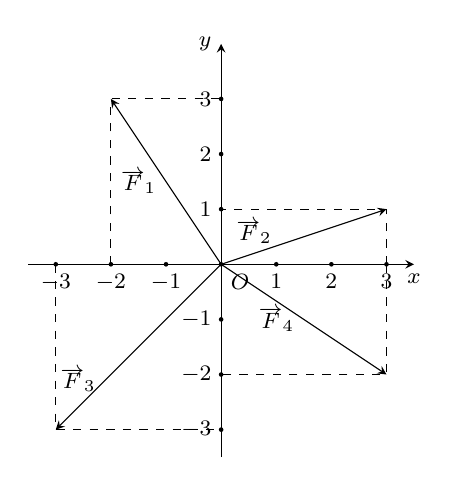
\begin{tikzpicture}[>=stealth,x=1cm,y=1cm,scale=0.7,font=\footnotesize]
			\draw[->] (-3.5,0) -- (3.5,0) node[below] {$x$};
			\draw[->] (0,-3.5) -- (0,4) node[left] {$y$};
			\fill (0,0) circle (1.2pt) node[below right]{$O$};
			\draw[-stealth](0,0)--(-2,3) node[pos=0.5,left]{$\overrightarrow{F}_1$};
			\draw[-stealth](0,0)--(3,1) node[pos=0.2,above]{$\overrightarrow{F}_2$};
			\draw[-stealth](0,0)--(-3,-3) node[pos=0.7,left]{$\overrightarrow{F}_3$};
			\draw[-stealth](0,0)--(3,-2) node[pos=0.5,left]{$\overrightarrow{F}_4$};			
			\foreach \a in {-3,-2,-1,1,2,3} \fill (\a,0) circle (1.2pt)node[below]{$\a$};		
			\foreach \b in {-3,-2,-1,1,2,3} \fill (0,\b) circle (1.2pt)node[left]{$\b$};
			\draw[dashed](-2,0)--(-2,3)--(0,3) (3,0)--(3,1)--(0,1)(3,0)--(3,-2)--(0,-2) (-3,0)--(-3,-3)--(0,-3);	 
		\end{tikzpicture}
	}
	\choice
	{(I)}
	{(II)}
	{(III)}
	{(IV)}
	\loigiai{
		Ta có $\vec{F} = \vec{F}_1 + \vec{F}_2 + \vec{F}_3 + \vec{F}_4 = \vec{i} - \vec{j}$.\\
		Dựa vào hệ trục tọa độ $Oxy$ ta thấy hợp lực nằm trong góc phần tư thứ tư.
	}
\end{ex}

%%==========Câu 9
\begin{ex}%[0H9H2-4]
	Trong mặt phẳng tọa độ $Oxy$, cho hai điểm $A(2 ;-1)$ và $B(-2 ; 1)$. Toạ độ điểm $M$ thuộc trục hoành và có hoành độ dương sao cho tam giác $ABM$ vuông tại $M$ là
	\choice
	{$M(\sqrt{5} ; 0)$}
	{$M(\sqrt{3} ; 0)$ và $M(-\sqrt{3} ; 0)$}
	{$M(-\sqrt{5} ; 0)$}
	{$M(-\sqrt{5} ; 0)$ và $M(\sqrt{5} ; 0)$}
	\loigiai{
		Gọi tọa độ $M(m; 0)$ thuộc trục $Ox$ với $m > 0$.\\
		Ta có $\vec{AM} = (m - 2; 1)$, $\vec{BM} = (m + 2; -1)$.\\
		Do $\triangle ABM$ vuông tại $M$ nên
		\[\vec{AM} \cdot \vec{BM} = 0 \Leftrightarrow m^2 - 4 -1 = 0 \Leftrightarrow \hoac{&m = \sqrt{5}\\& m = -\sqrt{5}.}\]
		Vậy tọa độ $M(\sqrt{5} ; 0)$.
	}
\end{ex}
%%==========Câu 10
\begin{ex}%[0H9V1-3]
	Cho tam giác $ ABC$ có $ A\left(5;3\right)$, $B\left(2;-1\right)$ và $C\left(-1;5\right)$. Toạ độ trực tâm $ H$ của tam giác $ ABC$ là
	\choice
	{$ H\left(-3;2\right)$}
	{$ H\left(-3;-2\right)$}
	{\True $ H\left(3;2\right)$}
	{$ H\left(3;-2\right)$}
	\loigiai{
		Gọi $AE$, $BK$ lần lượt là đường cao trong tam giác $ ABC$.\\
		Đường thẳng $AE$ đi qua điểm $ A\left(5;3\right)$ và có véc-tơ pháp tuyến $\overrightarrow{n}=\overrightarrow{BC}=\left(-3;6\right)=-3\left(1;-2\right)$.\\
		Nên $AE$ có phương trình tổng quát là\\ $1\left(x-5\right)-2\left(y-3\right)=0\Leftrightarrow x-2y+1=0$.\\
		Đường thẳng $BK$ đi qua điểm $B\left(2;-1\right)$ và có véc-tơ pháp tuyến $\overrightarrow{n}=\overrightarrow{AC}=\left(-6;2\right)=-2\left(3;-1\right)$.\\
		Nên $BK$ có phương trình tổng quát là $3\left(x-2\right)-\left(y+1\right)=0\Leftrightarrow 3x-y-7=0$ .\\
		Suy ra tọa độ điểm $H=AE\cap BK$ là nghiệm của hệ phương trình 
		$\heva{&x-2y+1=0\\ & 3x-y-7=0}
		\Leftrightarrow
		\heva{&x=3\\ & y=2.}$\\
		Vậy $ H\left(3;2\right)$.}
\end{ex}
%%==========Câu 11
\begin{ex} %[0H9H3-2]
	Trong mặt phẳng toạ độ, cho tam giác có $A\left(1;2\right)$, $B\left(3;1\right)$ và $C\left(5;4\right)$. Viết phương trình tổng quát của đường cao kẻ từ $A$ là
	\choice
	{$3x-2y-5=0$}
	{$3x-2y-5=0$}
	{$5x-6y+7=0$}
	{\True $3x+2y-8=0$}
	\loigiai{
		Đường cao $AH$ đi qua điểm $A\left(1;2\right)$ và có véc-tơ pháp tuyến $\overrightarrow{n}=\overrightarrow{BC}=\left(2;3\right)$.\\
		Vậy $AH$ có phương trình tổng quát là $2\left(x-1\right)+3\left(y-1\right)=0\Leftrightarrow 2x+3y-8=0$.
	}
\end{ex}
%%==========Câu 12
\begin{ex}%[0H9H3-2]
	Trong mặt phẳng toạ độ, cho đường thẳng $d$ đi qua hai điểm $A$, $B$. Đường thẳng $\Delta$ đi qua $C$ và song song với đường thẳng $d$.\\
	\begin{center}
		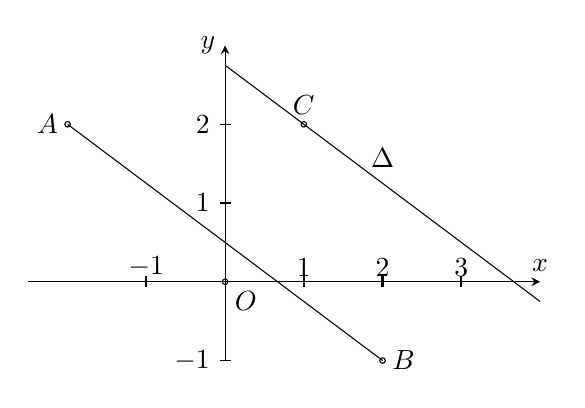
\begin{tikzpicture}[>=stealth]
			\draw[->](-2.5,0)--(4,0);
			\foreach \x in {-1,1,2,3}
			\draw[shift={(\x,0)},color=black,thick] (0pt,2pt) -- (0pt,-2pt) node[above] { $\x$};
			\draw[->](0,-1)--(0,3);
			\foreach \y in {1,2,-1}
			\draw[shift={(0,\y)},color=black] (2pt,0pt) -- (-2pt,0pt) node[left] {\normalsize $\y$};
			\draw (0,0) circle (1pt) node[below right] { $O$} ;
			\draw (4,0) node[above]{$x$} (0,3)
			node[left]{$y$};
			\coordinate (A)at(-2,2);
			\coordinate (B)at(2,-1);
			\coordinate (C)at(1,2);
			\coordinate (D)at(4,-1/4);
			\coordinate (E)at(0,11/4);
			\draw (-2,2) circle (1pt) node[left] { $A$} ;
			\draw (2,-1) circle (1pt) node[right] { $B$} ;
			\draw (1,2) circle (1pt) node[above] { $C$} ;
			\draw (2,4/3) node[above] {$\Delta$} ;
			\draw[black] (A)--(B);
			\draw[black] (E)--(D);
		\end{tikzpicture}
	\end{center}
	Phương trình của đường thẳng $\Delta$ là
	\choice
	{\True $3x+4y-11=0$}
	{$3x+4y-2=0$}
	{$4x-3y+2=0$}
	{$4x-3y+14=0$}
	\loigiai{
		Quan sát hình vẽ ta có $A\left(-2;2\right)$, $B\left(2;-1\right)$ và $C\left(1;2\right)$.\\
		Đường thẳng $\Delta$ đi qua điểm $C\left(1;2\right)$ và song song với đường thẳng $d$ có véc-tơ chỉ phương $\overrightarrow{u}=\overrightarrow{AB}=\left(4;-3\right)$ $\Rightarrow$ véc-tơ pháp tuyến $\overrightarrow{n}=\left(3;4\right)$ có phương trình là\\
		$3\left(x-1\right)+4\left(y-2\right)=0\Leftrightarrow 3x+4y-11=0$.}
\end{ex}
\Closesolutionfile{ans}
\bangdapan{0-Deso5-CD-GHKII-NH23-24}
\subsection{Câu trắc nghiệm đúng sai}
Học sinh trả lời từ câu 1 đến câu 4.
Trong mỗi ý \circlenum{A}, \circlenum{B}, \circlenum{C} và \circlenum{D} ở mỗi câu, học sinh chọn đúng hoặc sai.
\setcounter{ex}{0}
\LGexTF
\Opensolutionfile{ansbook}[ansbook/0-Deso5-CD-GHKII-NH23-24-DS]
\Opensolutionfile{ans}[Ans/0-Deso5-CD-GHKII-NH23-24-T]
%%%============EX_1==============%%%
\begin{ex}%[0D8V2-4]%[Dự án đề kiểm tra Toán khối 10 - GHK2 NH23-24-Dot 2- Đoàn Thanh Phong]%[Deso5- Sach CD]
	Một trường cấp $3$ của tỉnh Đồng Tháp có $8$ giáo viên Toán gồm có $3$ nữ và $5$ nam, giáo viên Vật lý thì có $4$ giáo viên nam, chọn ra một đoàn thanh tra công tác ôn thi THPTQG, khi đó
	\choiceTF
	{\True Chọn $1$ giáo viên nữ có $\mathrm{C}_3^1$ cách}
	{\True Chọn $2$ giáo viên nam môn Vật lý có $\mathrm{C}_4^2$ cách}
	{Chọn $1$ giáo viên nam môn Toán và $1$ nam môn Vật lý có $\mathrm{C}_5^1+\mathrm{C}_4^1$ cách}
	{Có $80$ cách chọn ra một đoàn thanh tra công tác ôn thi THPTQG gồm $3$ người có đủ $2$ môn Toán và Vật lý và phải có giáo viên nam và giáo viên nữ trong đoàn} 
	\loigiai{
		Vì chọn ra $3$ người mà yêu cầu phải có giáo viên nam và giáọ viên nữ trong đoàn nên số giáo viên nữ được chọn chỉ có thể bằng $1$ hoặc $2$.\\
		Ta xét hai trường hợp\\
		Trường hợp 1: Chọn $1$ giáo viên nữ: Có $\mathrm{C}_3^1$ cách. Khi đó:\\
		- Chọn $1$ giáo viên nam môn Toán và $1$ nam môn Vật Lý có $\mathrm{C}_5^1\cdot \mathrm{C}_4^1$. \\
		- Chọn $2$ giáo viên nam môn Vật lý có $\mathrm{C}_4^2$ cách.\\
		Trường hợp 2: Chọn $2$ giáo viên nữ có $\mathrm{C}_3^2$ cách chọn. Khi đó chọn thêm $1$ giáo viên nam môn Vật lý có $\mathrm{C}_4^1$ cách. Trường hợp này có $\mathrm{C}_3^2 \cdot \mathrm{C}_4^1$ cách chọn.\\
		Vậy tất cả có $\mathrm{C}_3^1\left(\mathrm{C}_5^1 \cdot  \mathrm{C}_4^1+\mathrm{C}_4^2\right)+\mathrm{C}_3^2 \cdot \mathrm{C}_4^1=90$ cách chọn.
	}
\end{ex}
%%%============EX_2==============%%%
\begin{ex}%[0D8H3-4]%[Dự án đề kiểm tra Toán khối 10 - GHK2 NH23-24-Dot 2- Đoàn Thanh Phong]%[Deso5- Sach CD]
	Khai triển $P=(x-\sqrt{3})^5$. Khi đó
	\choiceTF
	{Hệ số của $x^4$ trong khai triển là $5\sqrt{3}$}
	{\True Hệ số của $x^2$ trong khai triển là $-30\sqrt{3}$}
	{\True Hệ số của $x^3$ trong khai triển là $30$}
	{\True Hệ số của $x$ trong khai triển là $45$} 
	\loigiai{
		Ta có
		\begin{eqnarray*}
			P&=&(x-\sqrt{3})^5\\
			&=&\mathrm{C}_5^0 x^5+\mathrm{C}_5^1 x^4\left(-\sqrt{3}\right)+\mathrm{C}_5^2 x^3\left(-\sqrt{3}\right)^2+\mathrm{C}_5^3 x^2\left(-\sqrt{3}\right)^3 +\mathrm{C}_5^4 x\left(-\sqrt{3}\right)^4+\mathrm{C}_5^5\left(-\sqrt{3}\right)^5\\
			&=& x^5-5 \sqrt{3} x^4+30 x^3-30 \sqrt{3} x^2+45 x-9 \sqrt{3} .
		\end{eqnarray*}
		Hệ số của $x^4$ trong khai triển là $-5\sqrt{3}$.
	}
\end{ex}
%%%============EX_3==============%%%
\begin{ex}%[0H9N1-2]%[Dự án đề kiểm tra Toán khối 10 - GHK2 NH23-24-Dot 2- Đoàn Thanh Phong]%[Deso5- Sach CD]
	Cho $\overrightarrow{a}=3\overrightarrow{i}+2\overrightarrow{j}$, $\overrightarrow{b}=\overrightarrow{i}-\overrightarrow{j}$.
	\choiceTF
	{$\overrightarrow{a}=(3;-2)$}
	{$\overrightarrow{b}=(-1;1)$}
	{\True $2\overrightarrow{a}+3\overrightarrow{b}=(9;1)$}
	{\True $\overrightarrow{a}-2\overrightarrow{b}=(1;4)$} 
	\loigiai{
		\begin{itemize}
			\item $\overrightarrow{a}=(3;2)$.
			\item $\overrightarrow{b}=(1;-1)$.
			\item $\heva{&2\overrightarrow{a}=(6;4)\\&3\overrightarrow{b}=(3;-3)} \Rightarrow 2\overrightarrow{a}+3\overrightarrow{b}=(9;1)$.
			\item $-2\overrightarrow{b}=(-2;2) \Rightarrow \overrightarrow{a}-2\overrightarrow{b}=(1;4)$.
		\end{itemize}	
	}
\end{ex}
%%%============EX_4==============%%%
\begin{ex}%[0H9V3-2]%[Dự án đề kiểm tra Toán khối 10 - GHK2 NH23-24-Dot 2- Đoàn Thanh Phong]%[Deso5- Sach CD]
	Cho tam giác $ABC$ có phương trình của đường thẳng $BC$ là $7x+5y-8=0$, phương trình các đường cao kẻ từ $B$, $C$ lần lượt là $9x-3y-4=0$, $x+y-2=0$.
	\choiceTF
	{\True Điểm $B$ có tọa độ là $\left(\dfrac{2}{3} ; \dfrac{2}{3}\right)$}
	{\True Điểm $C$ có toạ độ là $(-1 ; 3)$}
	{Phương trình đường cao kẻ từ $A$ là $5x-7y-6=0$}
	{Phương trình đường trung tuyến kẻ từ $A$ là $x-13y+4=0$} 
	\loigiai{
		\begin{itemize}
			\item Tọa độ của điểm $B$ là nghiệm của hệ phương trình $\heva{&7x+5y-8=0\\&9x-3y-4=0}\Leftrightarrow\heva{&x=\dfrac{2}{3}\\&y=\dfrac{2}{3}.}$\\
			Suy ra điểm $B$ có tọa độ là $\left(\dfrac{2}{3} ; \dfrac{2}{3}\right)$
			\item Toạ độ của điểm $C$ là nghiệm của hệ phương trình $\heva{&7x+5y-8=0\\&x+y-2=0}\Leftrightarrow\heva{&x=-1\\&y=3.}$\\
			Suy ra điểm $C$ có toạ độ là $(-1 ; 3)$.
			\item Đường thẳng $AB$ đi qua điểm $B\left(\dfrac{2}{3};\dfrac{2}{3}\right)$ và nhận vec-tơ chỉ phương $\overrightarrow{u_1}(1;-1)$ của đường cao kẻ từ  $C$ làm vec-tơ pháp tuyến có phương trình là $$(x+1)+3(y-3)=0 \Leftrightarrow x+3y-8=0.$$
			Toạ độ của điểm $A$ là nghiệm của hệ phương trình $\heva{&x-y=0\\&x+3y-8=0}\Leftrightarrow\heva{&x=2\\&y=2.}$\\
			Suy ra điểm $A$ có tọa độ là $(2;2)$.\\
			Phương trình đường cao kẻ từ  $A(2;2)$ và nhận vec-tơ chỉ phương $\overrightarrow{u}(5;-7)$ của đường thẳng $BC$ làm vec-tơ pháp tuyến là $$5(x-2)-7(y-2)=0 \Leftrightarrow 5x-7y+4=0.$$
			\item Gọi $I$ là trung điểm của $BC$, ta có tọa độ của điểm $I$ là $\left(\dfrac{-1}{6};\dfrac{11}{6}\right)$.\\
			Do đó, ta có $\overrightarrow{IA}\left(\dfrac{13}{6};\dfrac{1}{6}\right)$.\\
			Đường trung tuyến kẻ từ  $A$ nhận $\overrightarrow{n}(1;-13)$ làm vec-tơ pháp tuyến có phương trình là $$(x-2)-13(y-2)=0 \Leftrightarrow x-13y+24=0.$$
		\end{itemize}
	}
\end{ex}
\Closesolutionfile{ans}
\Closesolutionfile{ansbook}
\begin{center}
	\textbf{\textsf{BẢNG ĐÁP ÁN ĐÚNG SAI}}
\end{center}
\input{Ansbook/0-Deso5-CD-GHKII-NH23-24-DS}

\subsection{Phần tự luận}
\hienthiloigiaibt
%%%=============BT_1=============%%%
\begin{bt}%[0D8V1-1]%[Dự án đề kiểm tra Toán khối 10 GHKII NH23-24-Dot 2-Dương Quang]%[Deso 5 - CD]
	Có bao nhiêu số tự nhiên có hai chữ số mà các chữ số hàng chục lớn hơn chữ số hàng đơn vị?
	\loigiai{
		Nếu chữ số hàng chục là $1$ thì chữ số hàng đơn vị là $0$, có $1$ số tự nhiên thỏa mãn.\\
		Nếu chữ số hàng chục là $2$ thì chữ số hàng đơn vị $0$ hoặc $1$, có $2$ số tự nhiên thoả mãn.\\
		Nếu chữ số hàng chục là $3$ thì chữ số hàng đơn vị là $0$ hoặc $1$ hoặc $2$, có $3$ số tự nhiên thỏa mãn.\\
		Theo quy luật đó, ta có số các số tự nhiên thóa mãn là $1+2+3+4+5+6+7+8+9=45$. 
	}
\end{bt}
%%%==============BT_2==============%%%
\begin{bt}%[0D8V2-4]%[Dự án đề kiểm tra Toán khối 10 GHKII NH23-24-Dot 2-Dương Quang]%[Deso 5 - CD]
	Lớp 11D có $45$ bạn học sinh. Đầu năm cô giáo muốn chọn ra một ban cán sự lớp từ $45$ bạn học sinh lớp 11D gồm một lớp trưởng, một lớp phó học tập, một lớp phó lao động và hai thư kí. Số cách cô giáo chọn ra một ban cán sự lớp như vậy là bao nhiêu?
	\loigiai{
		Để chọn ra ban cán sự lớp thoả mãn yêu cầu, ta tiến hành như sau:
		\begin{itemize}
			\item Bước $1$: Chọn $3$ bạn trong đó có một lớp trưởng, một lớp phó học tập, một lớp phó lao động từ $45$ bạn.\\
			Mỗi một cách chọn ra một ban cán sự lớp gồm ba bạn trong đó có một lớp trưởng, một lớp phó học tập, một lớp phó lao động từ $45$ bạn học sinh lớp 11D tương ứng với một chỉnh hợp chập $3$ của $45$ phần tử.\\
			Do đó số cách chọn là $\mathrm{A}_{45}^3$.
			\item Bước $2$: Chọn $2$ bạn làm thư kí từ $42$ bạn còn lại.\\
			Mỗi cách chọn này không phân biệt về thứ tự nên số cách chọn là $ \mathrm{C}_{42}^2$.
		\end{itemize}
		Số cách cô giáo chọn ra một ban cán sự lớp thoả mãn là $\mathrm{A}_{45}^3\cdot \mathrm{C}_{42}^2=73\,305\,540$. 
	}
\end{bt}
%%%==============BT_3==============%%%
\begin{bt}%[0D8H3-5]%[Dự án đề kiểm tra Toán khối 10 GHKII NH23-24-Dot 2-Dương Quang]%[Deso 5 - CD]
	Cho biểu thức $(1-x)^6$. Tính tổng $S=\mathrm{C}_6^0-\mathrm{C}_6^1+\mathrm{C}_6^2-\mathrm{C}_6^3+\mathrm{C}_6^4-\mathrm{C}_6^5+\mathrm{C}_6^6$.
	\loigiai{
		Ta có: $(1-x)^6=\mathrm{C}_6^0-\mathrm{C}_6^1x+\mathrm{C}_6^2x^2-\mathrm{C}_6^3x^3+\mathrm{C}_6^4x^4-\mathrm{C}_5^5x^5+\mathrm{C}_6^6x^6$. \hfill$(*)$\\
		Thay $x=1$ vào $(*)$, ta được 
		\[(1-1)^6=\mathrm{C}_6^0-\mathrm{C}_6^1+\mathrm{C}_6^2-\mathrm{C}_6^3+\mathrm{C}_6^4-\mathrm{C}_6^5+\mathrm{C}_6^6=S.\]
		Vậy $S=0$.
	}
\end{bt}
%%%==============BT_4==============%%%
\begin{bt}%[0H9C3-6]%[Dự án đề kiểm tra Toán khối 10 GHKII NH23-24-Dot 2-Dương Quang]%[Deso 5 - CD]
	Trong mặt phẳng tọa độ $Oxy$ cho hai điểm $A(1;-1)$ và $B(3;2)$. Tọa độ điểm $M$ thuộc trục $Oy$ để $MA^2+MB^2$ nhỏ nhất.
	\loigiai{
		Ta có $M\in Oy$ nên $M(0; m)$ và $\heva{&\overrightarrow{MA}=(1;-1-m) \\
			&\overrightarrow{MB}=(3; 2-m).
			&}$\\
		Khi đó $MA^2+MB^2=\left|\overrightarrow{M A}\right|^2+\left|\overrightarrow{M B}\right|^2=2\left(m-\dfrac{1}{2}\right)^2+\dfrac{29}{2} \geq \dfrac{29}{2}, \forall m \in \mathbb{R}$.\\
		Suy ra giá trị nhỏ nhất của $MA^2+MB^2$ bằng $\dfrac{29}{2}$ khi $m=\dfrac{1}{2} \Rightarrow M\left(0; \dfrac{1}{2}\right)$.
	}
\end{bt}
%%%==============BT_5==============%%%
\begin{bt}%[0H9C3-5]%[Dự án đề kiểm tra Toán khối 10 GHKII NH23-24-Dot 2-Dương Quang]%[Deso 5 - CD]
	Viết phương trình đường thẳng $\Delta$ đi qua $A(5;1)$ và cách điểm $B(2;-3)$ một khoảng bằng $5$.
	\loigiai{
		Gọi $\overrightarrow{n}=(a; b)$ là vectơ pháp tuyến của đường thẳng $\Delta$.\\ 
		$\Delta$ đi qua $A(5; 1)$ nên có phương trình 
		\begin{eqnarray*}
			&& a(x-5)+b(y-1)=0\\
			&\Leftrightarrow&ax+by-5a-b=0.
		\end{eqnarray*}
		Ta có
		\begin{eqnarray*}
			\mathrm{d}(B, \Delta)=5 &\Leftrightarrow&  \dfrac{|2 a-3 b-5 a-b|}{\sqrt{a^2+b^2}}=5 \\
			&\Leftrightarrow&  |-3 a-4 b|=5 \sqrt{a^2+b^2} \\
			&\Leftrightarrow&  (3a+4b)^2=25\left(a^2+b^2\right) \\
			&\Leftrightarrow&  9a^2+24a b+16b^2=25a^2+25b^2 \\
			&\Leftrightarrow&  16a^2+9b^2-24a b=0 \\
			&\Leftrightarrow&  (4a-3b)^2=0 \\
			&\Leftrightarrow&  4a-3b=0 \\
			&\Leftrightarrow& 	4a=3b.
		\end{eqnarray*}
		Chọn $a=3\Rightarrow b=4$. Ta có phương trình $\Delta\colon 3x+4y-19=0$.
	}
\end{bt}
%%%==============BT_6==============%%%
\begin{bt}%[0H9V3-4]%[Dự án đề kiểm tra Toán khối 10 GHKII NH23-24-Dot 2-Dương Quang]%[Deso 5 - CD]
	Cho hai đường thẳng $\Delta_1\colon ax-y+5=0$ và $\Delta_2\colon x+y+1=0$. Có bao nhiêu giá trị của $a$ để $\Delta_1$ tạo với $\Delta_2$ một góc $60^\circ$.
	\loigiai{
		Ta có $\overrightarrow{n}_1(a;-1)$ và $\overrightarrow{n}_2(1; 1)$.\\ 
		Theo bài ra $\Delta_1$ tạo với $\Delta_2$ một góc $60^{\circ}$ nên
		\begin{eqnarray*}
			\cos\left(\Delta_1,\Delta_2\right)=\dfrac{\left|\overrightarrow{n}_1\cdot\overrightarrow{n}_2\right|}{\left|\overrightarrow{n}_1\right|\cdot\left|\overrightarrow{n}_2\right|}
			&\Leftrightarrow& \cos 60^{\circ}=\dfrac{|a-1|}{\sqrt{a^2+(-1)^2} \cdot \sqrt{1^2+1^2}}\\
			&\Leftrightarrow& \dfrac{1}{2}=\dfrac{|a-1|}{\sqrt{2} \cdot \sqrt{a^2+1}}  \\
			&\Leftrightarrow&  \sqrt{a^2+1}=\sqrt{2}|a-1| \\
			&\Leftrightarrow&  a^2-4 a+1=0 \\
			&\Leftrightarrow&  \hoac{&a=2+\sqrt{3} \\
				&a=2-\sqrt{3}.
				&} \\
		\end{eqnarray*}
		Vậy có hai giá trị của $a$ thỏa mãn.
	}
\end{bt}